%
The 7447 IC helps in displaying decimal numbers on the seven segment display.  The $\bar{a}-\bar{f}$, pins of the 7447 IC are connected to the $a-f$ pins of the display. $V_{cc}$ should be connected to a 5V power source. The input pins of the decoder are A,B,C and D, with A being the lowest significant bit (LSB) and D being the most significant bit (MSB).  For example, the number 5 is visible on the display when the A,B,C and D inputs are the following.
\begin{center}
	\begin{tabular}{|c|c|c|c|c|}
\hline
D & C & B & A & Decimal
\\ \hline
0 & 1 & 0 & 1 & 5
\\
\hline
\end{tabular}
\end{center}
%
\begin{figure}[!h]
\begin{center}
\resizebox {\columnwidth} {!} {
\input{./figs/7447.tex}
}
\end{center}
\caption{}
\label{fig:7447}
\end{figure}

%%
%\begin{figure}[!h]
%\begin{center}
%\includegraphics[width=\columnwidth]{./figs/7447IC}
%\end{center}
%\caption{}
%\label{}
%\end{figure}

%\begin{center}
	%\includegraphics[scale=1.5]{7447IC}
%\end{center}

%
\begin{problem}
	Connect the 7447 IC decoder $\bar{a}-\bar{g}$ pins to the $a-g$ pins of the display respectively.
\end{problem}
\begin{problem}
	Connect the $V_{cc}$ and GND pins of the decoder to the 5V supply and GND pins of the breadboard.
\end{problem}

\subsection{Driving the Segments}
\begin{problem}
Connect the A-D pins of the 7447 IC to the pins D2-D5 of the Arduino.
\end{problem}	
\begin{problem}
Type the following code and execute. What do you observe? 
%Explain  through Fig. \ref{fig:Atmega168PinMap2}
\lstinputlisting[language=C]{./codes/7447/decoder.asm}
%\input{ard_decoder_drive}
\end{problem}
%
\begin{problem}
Now generate the numbers 0-9 by modifying the above program.
\end{problem}
%
%\begin{figure}[!h]
%\begin{center}
%\includegraphics[width=\columnwidth]{./figs/Atmega168PinMap2}
%\end{center}
%\caption{}
%\label{fig:Atmega168PinMap2}
%\end{figure}
%\newpage

\section{Boolean Operations}
%
Test all the following using the 7447 IC
\begin{problem}
Verify the AND,OR and XOR operations in assembly.
\end{problem}
\solution
\lstinputlisting[language=C]{./codes/boolean/and_or_xor.asm}
\begin{problem}
\label{prob:ch2_complement}
Write a routine for finding the complement of a number.
\end{problem}
\solution
\lstinputlisting[language=C]{./codes/boolean/complement.asm}
%\subsection{Counting Decoder}
%
%\begin{problem}
%Write an assembly program for the AND operation.  
%\end{problem}
%\solution
%\lstinputlisting[language=C]{./codes/logic_and}
%%
%\begin{problem}
%Write an assembly program for the OR operation.  
%\end{problem}
%\solution
%\lstinputlisting[language=C]{./codes/logic_or}
%%
%\begin{problem}
%Write an assembly program for the XOR operation.  
%\end{problem}
%\solution
%\lstinputlisting[language=C]{./codes/logic_xor}
%%
%\begin{problem}
%Write an assembly program to complement a bit using the XOR operation.
%\end{problem}
%%
%%
%\begin{problem}
%Write an assembly routine to complement a bit. Call this routine by using RCALL.
%\end{problem}

%\solution
%\lstinputlisting[language=C]{./codes/complement}

%
%\begin{problem}
%Use the following code for LED blinking. You will have to connect pin 13 to the LED on the seven segment display.
%\end{problem}
%\lstinputlisting[language=C]{./codes/blink}
%%
%\begin{problem}
%Find the exact blinking delay for the above.  Verify your result through an oscilloscope. 
%\end{problem}
%%
%\begin{problem}
%Modify the above code to get the blinking delay to 1 second.  Verify your results.
%\end{problem}
%%
%\begin{problem}
%Implement a decade counter.
%\end{problem}

%The $\&\&$ operand is used for the boolean AND (multiplication) operation, the $||$ operand is used for the OR (addition) operation and the ! operand is used for the NOT ($^{'}$) operation in Arduino code.  For example, the expression for \eqref{bool_logic} in Arudino is
%\begin{verbatim}
%D = (W&&X&&Y&&!Z)||(!W&&!X&&!Y&&Z);
%\end{verbatim}
%\subsection{Display Decoder}
%%
%\begin{problem}
%Now write the truth table for the seven segment display decoder (IC 7447).  The inputs will be $A,B,C,D$ and the outputs will be $a,b,c,d,e,f,g$.
%\end{problem}
%%
%\begin{problem}
%\label{seven_seg_disp_logic}
%Obtain the logic functions for outputs $a,b,c,d,e,f,g$ in terms of the inputs $A,B,C,D$.
%\end{problem}
%\begin{problem}
%Disconnect the arduino from IC 7447 and connect the pins D2-D8 in the Arduino directly to the seven segment display.
%\end{problem}
%\begin{problem}
%Write a new program to implement the logic in Problem \ref{seven_seg_disp_logic} and observe the output in the display.  You have designed the logic for IC 7447!
%\end{problem}
%\begin{problem}
%Now include your counting decoder program in the  display decoder program
%and see if the display shows the consecutive number.
%\end{problem}
%A decade counter counts the numbers from 0-9 and then resets to 0.
%\begin{problem}
%Suitably modify the above program to obtain a decade counter.
%\end{problem}





%\begin{problem}
%Generate the boolean functions for the segments $a-f$ using the table in Problem \ref{bcd_ss}.  For example, the function for $a$ is obtained from the table as
%\begin{equation}
%a=\bar{D}\bar{C}\bar{B}A+\bar{D}C\bar{B}\bar{A}
%\label{boolean}
%\end{equation}
%\end{problem}
%%
%\begin{problem}
	%\label{counter_dec}
%Write functions for $A,B,C,D$ in Arduino using the following table and verify using the Arduino driven display.
		%\input{counter_decoder}
%\end{problem}
%\begin{problem}
	%Write a module for decimal to binary conversion
	%according to the example given below
	%\input{conversion}
	%%
	%$N \% 2$ gives the remainder and $N/2$ gives the quotient
%	and use it in the above code so that decimal values are given as input in the program and observed as output in the display. Note that the following code
%	\begin{verbatim}
%	a % b
%	\end{verbatim}
%	can be used to obtain the remainder when a is divided by b and
%	\begin{verbatim}
%	a/b
%	\end{verbatim}
%	gives the quotient.
%\end{problem}
